\chapter{Attack scenarios}\label{chap:attack scenarios}

The goal of this \namecref{chap:attack scenarios} is to give an overview of various attacks on Peras, which either motivate a Peras certain rule/requirement or highlight what we can expect from sufficiently strong attacker within our margin of security.

\section{Attacks against Peras}

Here, we list attacks that a sufficiently strong adversary (within the margin of security) can execute and degrade the user experience this way (for example, due to reduced throughput or longer settlement times), but which do not threaten the core security properties of the system.

\subsection{Abstaining during voting}\label{sec:abstaining during voting}

An adversary with $\alpha$ stake will have $\alpha\cdot\perasN$ votes on average, so if they simply abstain, the honest nodes will likely fail to reach quorum even when they all vote for the same block when $\alpha \ge 1-\perasQuorum\perasN = 1/4$ for $\perasQuorum = 3/4 \cdot \perasN$.
Therefore, Peras doesn't provide fast settlement in the presence of an adversary with $\alpha\ge 25\%$, which is expected.

As usual, this is assuming full honest participation; smaller participation levels can only tolerate proportionally weaker adversaries.

Additionally, this attack (and others that are about preventing a quorum) gets more effective if the cryptographic scheme used for certificates requires votes of weight larger than \perasQuorum{} to certify a quorum, which is for example the case for ALBA due to its $n_p/n_f$ parameters \parencite{chaidos2024approximate}.

\subsection{Honest vote splitting}\label{sec:honest vote splitting}

In the pre-alpha version of Peras, honest nodes vote for the newest block on their selection that is at least \perasBlockMinSlots{} slots old.%
\footnote{There are potential variants of this rule (such as choosing the tip of the best chain made out of blocks that at least \perasBlockMinSlots{} slots old) that might mitigate the attack discussed here in certain scenarios, but they do not change the overall picture.}
It is relatively easy for an adversary to cause different honest nodes to vote for different blocks.

For example, this allows an adversary with $\alpha<0.25$ to prevent quorum formation with decent probability (which they couldn't do by simply abstaining) by splitting the honest votes such that neither block reaches quorum, causing the system to enter a cooldown period.
Future versions of Peras will improve on this front by adding a dedicated \emph{pre-agreement} mechanism that \emph{avoids} a cooldown in this scenario.

Write $\operatorname{tip}(C)$ for the tip of a chain $C$, and $\operatorname{trunc}(s,C)$ for the prefix of $C$ up until (but excluding) slot $s$.

Concretely, consider the voting phase at the beginning of round $r$ starting in slot $s$, with all honest nodes having selected chain $C_1$ just before.

Suppose that the adversary with stake $\alpha$ has a chain $C_2$ that is preferrable to $C_1$, and $D_1 \neq D_2$ where \[D_i = \operatorname{tip}(\operatorname{trunc}(s-\perasBlockMinSlots,C_i))\] for $i\in\{1,2\}$.
If the adversary now diffuses $C_2$ to only a subset of the honest nodes right before $r$ starts (such that the remaining honest nodes only receive $C_2$ after $r$ began), these nodes will vote for $D_2$, while the rest will vote for $D_1$.

We can calculate a lower bound on the probability that an adversary has such a chain $C_2$ by considering a particular outcome of the leader schedule that guarantees the existence of $C_2$ when the adversary simply abstains while honest chain is growing before round $r$.

\begin{enumerate}
\item\label{enumi:honest vote splitting:a}
  There is at least one adversarial active slot in the interval $(h,s-\perasBlockMinSlots)$ where $h$ is the last honest active slot before $s-\perasBlockMinSlots$.
\item\label{enumi:honest vote splitting:b}
  There are at not more honest than adversarial active slots in the interval $[s-\perasBlockMinSlots, s)$.
\end{enumerate}
Condition~\ref{enumi:honest vote splitting:a} guarantees that $D_1\neq D_2$, and condition~\ref{enumi:honest vote splitting:b} makes sure that $C_2$ is preferrable to $C_1$.

We stress that this is not the only scenario where the attack can be executed; for example, we have not considered tiebreakers and honest short forks.

\begin{lemma}\label{lemma:honest vote splitting prob}
  For an adversary with stake $\alpha$ the probability that the events~\ref{enumi:honest vote splitting:a} and~\ref{enumi:honest vote splitting:b} occur before some Peras round is given by \[ P(H\le A) \cdot P(A' \ge 1) \]
  where $H\sim\operatorname{Binom}(L,\phi(1-\alpha))$, $A\sim\operatorname{Binom}(L,\phi(\alpha))$, $A' \sim \operatorname{Binom}(H',\phi(\alpha))$, $H' \sim \operatorname{Geom}(\phi(1-\alpha))$\footnote{Here, we use the convention of counting the number of failures until the first success.}, and where $L= \perasBlockMinSlots$ and $\phi(\sigma) = 1-{(1-\asc)}^\sigma$ \parencite[(1)]{david2018ouroboros}.
\end{lemma}
\begin{proof}
  Note that~\ref{enumi:honest vote splitting:a} and~\ref{enumi:honest vote splitting:b} are independent as they refer to disjoint sets of slots.

  The number of active slots out of $n$ total slots for a party with stake $\sigma$ is binomially distributed via $\operatorname{Binom}(n,\phi(\sigma))$, so $P(\enquote{\ref{enumi:honest vote splitting:a}}) = P(H\le A)$ is clear.

  The number of successive inactive slots until an active slot for a party with stake $\sigma$ is geometrically distributed via $\operatorname{Geom}(\phi(\sigma))$, so $H'$ counts the size of the interval $(h,s-L)$, and therefore $A' \sim \operatorname{Binom}(H',\phi(\alpha))$ counts the number of adversarial active slots in that interval.
  Thus, $P(\enquote{\ref{enumi:honest vote splitting:b}}) = P(A'\ge 1)$.
\end{proof}

In \cref{lemma:honest vote splitting prob}, we assume that the gap $H'$, i.e.\ the length of the interval $(h,s-\perasBlockMinSlots)$, is sampled geometrically due to the leader schedule.
However, it can also be instructive to set it to a concrete value (letting $H'$ have a one-point distribution), especially if an adversary could force a long gap in some other way.

\begin{figure}[h]
  % see honest-vote-splitting.py
  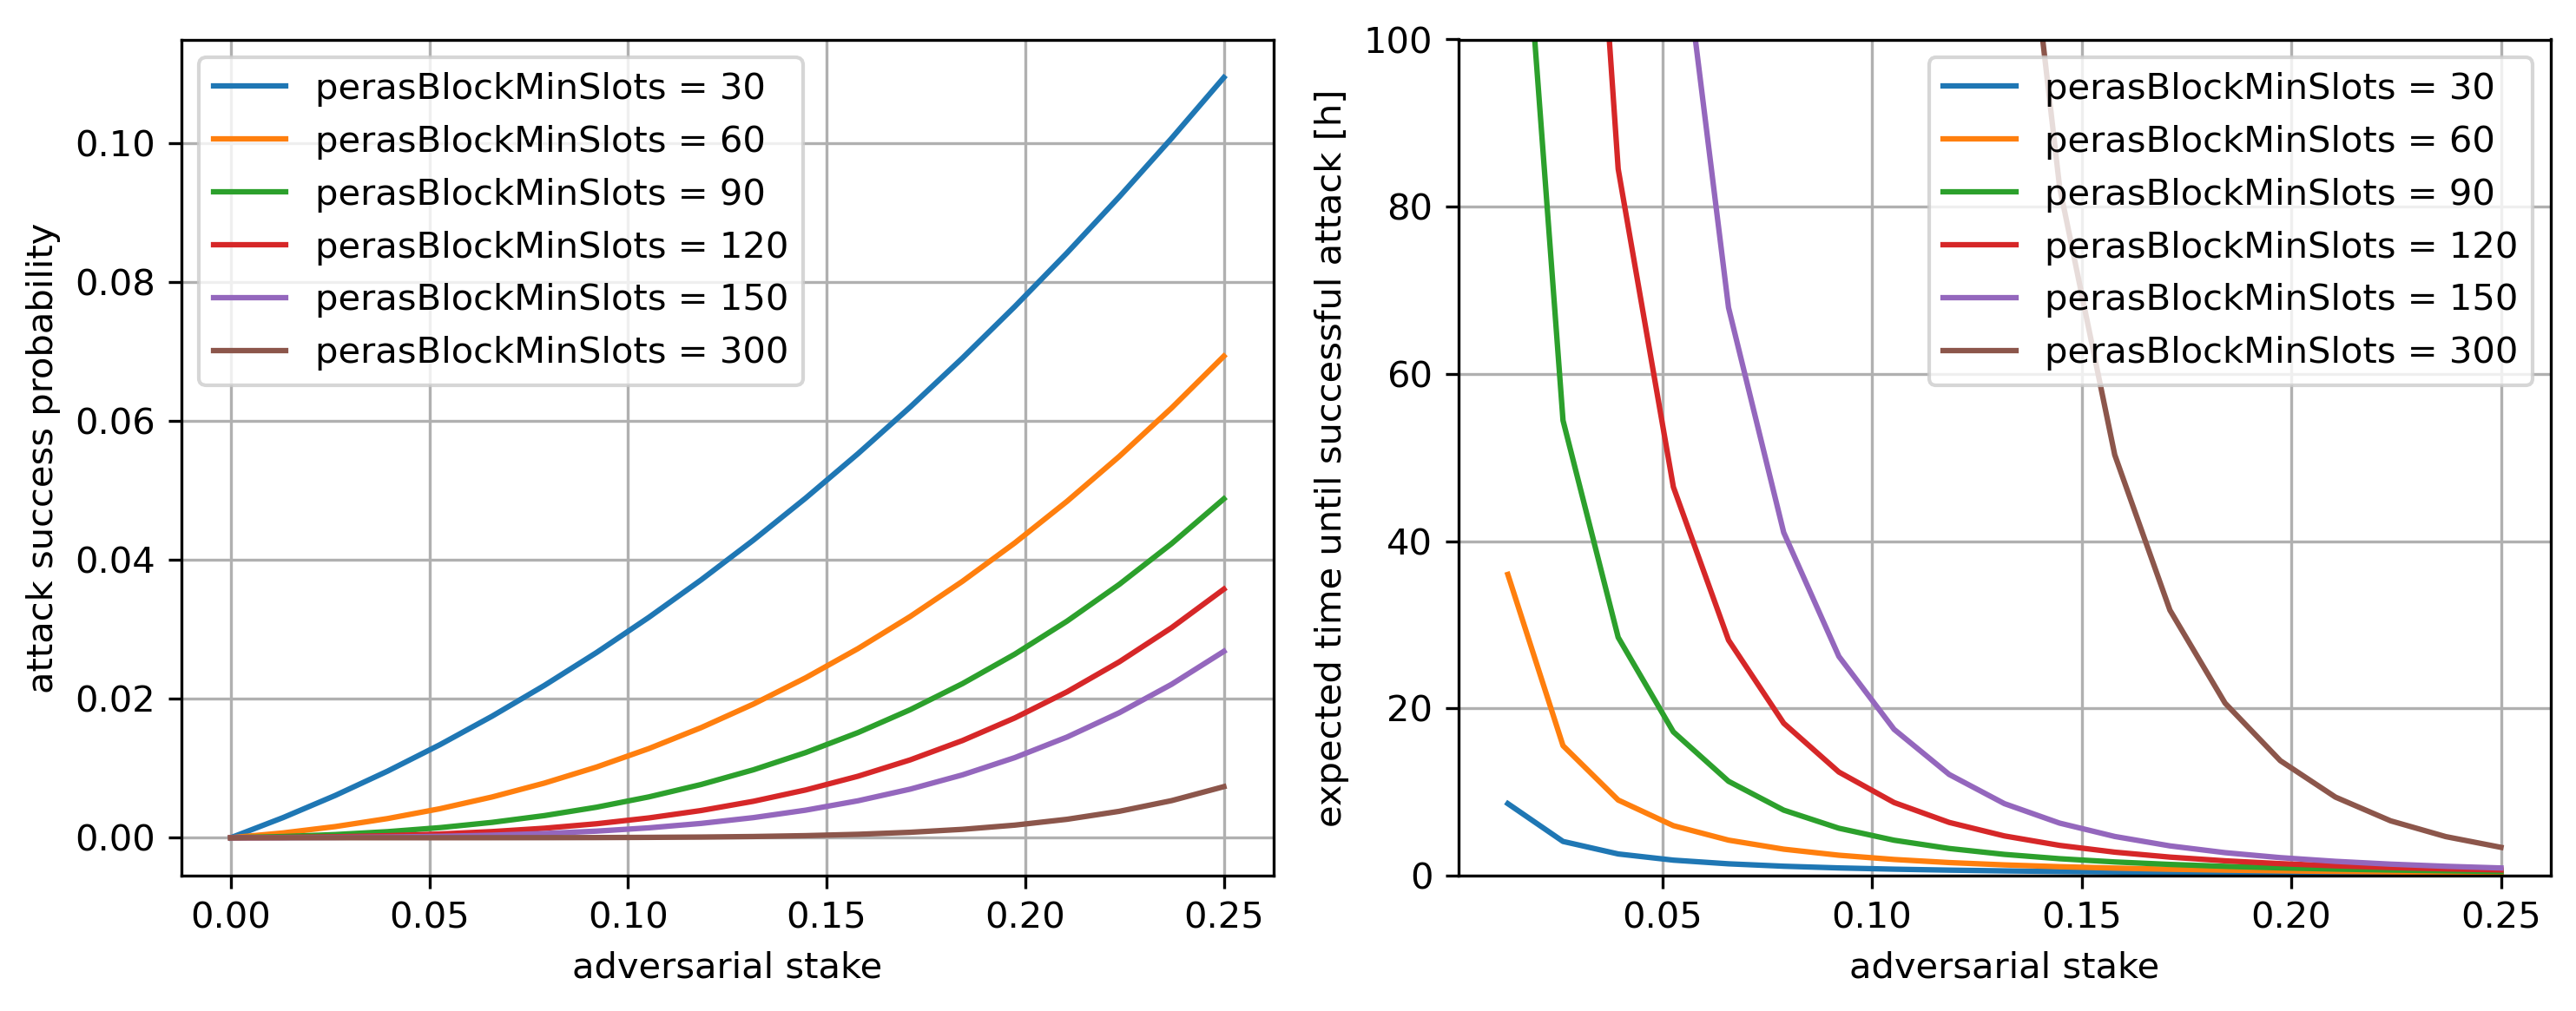
\includegraphics[width=0.95\textwidth]{./appendix/plot-honest-vote-splitting.png}
  \centering
  \caption{Probabilities (lower bounds) for \cref{lemma:honest vote splitting prob} for realistic parameters. The right plot assumes a slot length of one second and $\perasRoundSlots = 90$.}\label{fig:honest vote splitting prob}
\end{figure}
We plot the propabilities of \cref{lemma:honest vote splitting prob} for realistic parameters in \cref{fig:honest vote splitting prob}.
We observe that for small values for \perasBlockMinSlots{}, even relatively weak adversaries can execute a vote splitting attack rather frequently.
This is relevant in particular as it allows them to trigger a cooldown phase.

\subsection{Density reduction via boost-induced rollbacks}\label{sec:density reduction via boost-induced rollbacks}

We now describe an adversarial strategy that results in the honest historical chain to have low density, but high weight, i.e.\ in the extreme case, there is one boosted block per Peras round, with every voting round being successful.
In that case, a simple (private) fork purely made out of adversarial blocks has a good chance to have higher density (but significantly lower weight) than the honest chain.

See \cref{sec:weighted genesis} for how this attack influences the Peras design.

Consider a Peras round $r$ starting in slot $s$.
During round $r$, the adversary (with stake $\alpha$) does not diffuse any votes or blocks until shortly before the end of round $r$ in slot $s+\perasRoundSlots$.
Let $C$ be the best chain that any honest node has selected in slot $s+\perasRoundSlots-1$.
The adversary arranges it such that during the voting phase of round $r$, no quorum is reached without the adversarial votes, and further, that honest votes with weight at most $\perasQuorum - \alpha$ are cast for a block $B$ that is \emph{not} on $C$.
The idea now is for the adversary to diffuse its $\alpha\cdot\perasN$ votes for $B$ near the end of round $r$ such that round $r$ is considered successful and $B$ receives a boost.
Then, under reasonable assumptions, the chain ending in $B$ is preferrable to $C$ (as the latter doesn't contain a block that was boosted during round $r$), so the adversary succeeded in creating a low density but high weight chain during round $r$.

\medskip
Let us consider concretely how and under what conditions an attacker can execute this attack.
\begin{enumerate}
\item
  To start the attack, the attacker needs to prevent a quorum out of honest votes during round $r$, and needs to ensure that votes of weight at least $\perasQuorum - \alpha$ are cast for a block that the honest nodes will not build upon during round $r$.

  One way to accomplish this is to execute an honest vote splitting attack, see \cref{sec:honest vote splitting}.

  If $\alpha<0.25$, then the adversary must proceed exactly as described there, in particular, diffuse an appropriate chain right before round $r$ starts, in order to prevent a quorum purely made out of honest votes.
  On the other hande, if $\alpha\ge 0.25$, preventing an honest quorum is trivial, see \cref{sec:abstaining during voting}, so the adversary also has the option to diffuse the better chain even after $r$ started.
\item
  The round length \perasRoundSlots{} must not be too long in relation to \perasBoost{}, i.e.
  \[ \perasBoost \ge \phi(1-\alpha)\cdot \perasRoundSlots \;. \]
  Otherwise, the honest chain built during round $r$ might have more weight than the block $B$ (plus additional adversarial blocks on top of $B$) despite not having a boost.
  The attacker can still execute a less effective version of the attack by diffusing their votes signifcantly \emph{before} the end of round $r$.

  However, for realistic/useful Cardano mainnet parameters, such as $\perasRoundSlots = 90$ and $\perasBoost = 15$, this is not a problem for the adversary.
\item
  Once an adversary successfully performed the attack in a round, they can repeat it with good probability like this.
  The idea is for the adversary to mint two blocks $B_1,B_2$ on top of $B$ between slot $s-\perasBlockMinSlots$ and $s+\perasRoundSlots -\perasBlockMinSlots$, where $B_1$ is preferrable to $B_2$.
  Then, they execute an honest vote splitting attack between $B_1$ and $B_2$ for round $r+1$, such that neither block reaches quorum just due to honest votes, but such that $B_2$ votes having weight $\perasQuorum - \alpha$ at least.
  This is exactly the necessary setup to continue with the attack.

  The number of elections of a party with stake $\sigma$ within $n$ slots is given by
  \[ E_{n,\sigma}\sim\operatorname{Pois}(-n\sigma\log(1-\asc)) \]
  in the limiting case when the stake is distributed across infinitely many stake pools.
  Therefore, the probability that the adversary gets two elections in the aforementioned slot interval of size \perasRoundSlots{} is bounded by $P(E_{\perasRoundSlots,\alpha}\ge 2)$.
  For example, for $\perasRoundSlots = 90$ and $\alpha=0.4$, this evaluates to $55.09\%$.

  The number of successive successful rounds is hence geometrically distributed.
  Note that all blocks added to the chain in the meantime are adversarial, hence impacting chain quality.\footnote{However, such reductions in chain quality are not necessarily too unexpected in the presence of such strong adversaries, and the situation might overall still be better than with pure Praos.}
\end{enumerate}

These probabilities seem sufficiently large to us to take this attack seriously.
A more detailed analysis (potentially simulating the resulting Markov chain) is out-of-scope for this document.

\section{Attacks motivating aspects of the Peras design}

Here, we list attacks that motivate (and are hence prevented by) certain rules of the Peras design.

\subsection{Attack on a variant of the block creation rule}\label{sec:attack block creation rule}

Peras enters a \emph{cooldown period} when a round does not give rise to a certificate.
In order to coordinate the \emph{end} of the cooldown period, a certificate is included on chain.

When an honest node is elected in a slot in round $r$, it includes the latest certificate $\cert'$ it has seen if and only if all of the following hold:
\begin{enumerate}
\item\label{rule:block creation:a} The node has not seen a certificate $\cert$ with $\round(\cert)=r-2$.
\item\label{rule:block creation:b} $r-\round(\cert') \le \perasCertMaxRounds$.
\item\label{rule:block creation:c} $\round(\cert') > \round(\cert^*)$.
\end{enumerate}
Here, rule~\ref{rule:block creation:c} makes sure that an honest node never includes a certificate that has already been included in our current selection.
Rule~\ref{rule:block creation:b} allows us to disregard votes/certificates beyond a certain age.

Rule~\ref{rule:block creation:a} makes sure that all honest nodes have stopped voting, preventing useless certificate inclusions.
Concretely, rule~\ref{rule:block creation:a} implies that no honest node voted in round $r-1$, assuming that round $r-3$ was successful (i.e.\ we were not in a cooldown phase, so the voting rule (VR-2A) doesn't apply in round $r-1$).

To see this, we consider the contrapositive, i.e.\ assume that an honest node \emph{did} vote during round $r-1$.
Due to voting rule (VR-1A), it must have observed a certificate for round $r-2$ at the beginning of round $r-1$.
However, as $\perasRoundSlots\ge\perasDelta$, the votes for that certificate (including adversarial ones) must have been diffused to all honest nodes before round $r$.
Therefore, rule~\ref{rule:block creation:a} is not satisfied for any honest node during round $r$.\qed{}

In contrast, if we were to modify rule~\ref{rule:block creation:a} to be about the absence of a certificate in round $r-1$, then an adversary could force nodes to unnecessarily include a certificate on chain.
Concretely, the adversary can diffuse its votes shortly before the start of round $r$, such that some honest nodes see a quorum for round $r-1$, while others do not.
If the latter category of nodes is sufficiently small, then them not voting during round $r$ does not preclude the possibility of round $r$ being successful, in which case they will vote again in round $r$ as normal.
However, the modified rule~\ref{rule:block creation:a} would still force them to include the most recent certificate on chain when they are elected before they receive the adversarial votes for round $r-1$, which we want to avoid.

It may be useful to clarify that the harm of honest nodes unnecessarily including a certificate on chain is not necessarily the presence of the certificate itself.
Note that an adversary can include a certificate in any block they mint, for example, with the only risk being reputational harm.
Instead, the harm done by honest nodes including unnecessary certificates in the honest blocks they mint is that the limit on block size means the bytes occupied by the certificate could have otherwise been occupied by transactions.

\subsection{Adding weight to Genesis density comparisons}\label{sec:weighted genesis}

The implementation approach of Ouroboros Genesis in the Cardano node fundamentally relies on the following property, justified by the analysis of the Genesis chain selection rule in~\cite{badertscher2018ouroboros}:
\begin{tcolorbox}[title=\densityOfCompetingChainsName]\label{property:density-of-competing-chains}
  Let $p$ be any historical point on the honest chain. The honest chain of a net that has always executed Praos under nominal conditions will have strictly higher density in the \sgen{} slots immediately following $p$ than any alternative chain that intersects at $p$.
\end{tcolorbox}
Here, the \emph{density} of a chain in a range of slots is defined to be the number of blocks in that range.

\medskip
With Peras, it is natural to modify this property to talk about the \emph{weight} in the \sgen{} slots instead of just the number of blocks:
\begin{tcolorbox}[title=\weightedDensityOfCompetingChainsName]\label{property:weighted-density-of-competing-chains}
  Let $p$ be any historical point on the honest chain. The honest chain of a net that has always executed Peras under nominal conditions will have strictly higher weight in the \sgen{} slots immediately following $p$ than any alternative chain that intersects at $p$.
\end{tcolorbox}
In the implementation, relying on this rule instead of \densityOfCompetingChains{} results in additional complexity and operational costs:
\begin{itemize}
\item A syncing node must download certificates in order to perform Genesis density comparisons.
  This requires modifications to the existing Genesis logic, which currently gets by with looking purely at header chains.
\item Nodes need to store certificates boosting blocks on the historical/immutable chain stored indefinitely, such that they can be given to syncing peers.
  This increases disk and outbound bandwidth requirements.
\end{itemize}
However, this complexity is necessary, as \cref{sec:density reduction via boost-induced rollbacks} describes an attack that would be possible if we were to keep using \densityOfCompetingChains{} instead of implementing \weightedDensityOfCompetingChains{}.
Concretely, the adversary can use the attack to let the honest chain to have less than $\phi(\alpha) \cdot \sgen$ blocks (i.e.\ the average number of blocks on a chain they can create completely by themselves) in a window of $\sgen$ slots, despite having higher weight.
Once successful, the adversary can cause syncing nodes to commit to the adversarial chain permanently, violating safety.

\subsection{Spamming equivocating votes}\label{sec:attack equivocations}

The adversary can equivocate any of their seats in the voting committee of a Peras round by creating more than one vote for each seat, voting for different blocks.
An adversary with $\alpha<1/2$ stake can not use this to cause a quorum for different blocks in the same round due to the choice of $\perasQuorum = 3/4$ and a quorum intersection argument.

However, in a naive implementation, the adversary can use equivocating votes to cause unbounded additional network traffic for honest nodes.
Most directly, they can send many equivocating votes to any of their peers individually.
If this is disallowed (by requiring nodes to only forward the first vote per voting committee seat per round), the adversary can diffuse different equivocating votes to different peers, such that nodes still download many different equivocating votes from their peers.

We now describe how this can be avoided; specifically, honest nodes will only ever download at most one vote (or alternatively, a bounded amount of votes) per voting committee seat per round.

An honest node downloads votes from its peers in two stages:
\begin{enumerate}
\item\label{enumi:equivocation:step 1}
  In the first stage, it requests and downloads \emph{vote IDs} from its peers.

  The vote ID must be chosen as to uniquely identify a voting committee seat in a particular round.
  Concretely, it can be represented as the round number and a proof of eligibility, which might be the stake pool identity or a VRF proof.

  Also, we assume vote IDs to be significantly smaller than full votes.
\item\label{enumi:equivocation:step 2}
  In the second stage, the node downloads votes corresponding to all vote IDs \emph{without duplicates}.
  Upon receiving a vote, it is checked that the vote matches the supplied vote ID.\@

  This way, observing equivocating votes is impossible.
\end{enumerate}
As an optimization (for example to reduce the impact of slow peers), the same vote ID could also be requested from multiple peers (bounded by a small constant) in~\ref{enumi:equivocation:step 2}.
While possible and sound, it is not necessary to discard equivocating votes received this way.

Additionally, this approach requires us to diffuse of certificates in addition to votes in general (even between caught-up peers).
To see why, consider two honest nodes $H_1,H_2$ and an adversarial node $A$ which are pairwise connected.
Suppose that we are in round $r$, both $H_1$ and $H_2$ are only one vote short of a quorum for the block $B$ in round $r$, and all honest votes for round $r$ have already been diffused.
Now the adversary sends $H_1$ and $H_2$ a new vote ID $\mi{vid}$, and then equivocates $\mi{vid}$ to send a vote $v_B$ for $B$ to $A$, but a vote $v_{B'}$ for a block $B' \neq B$ to $A'$.
Now $A$ observes a quorum for $B$ in round $r$, creating a certificate, while $A'$ does not.
The vote diffusion mechanism described above causes $A'$ to not request a vote for $\mi{vid}$ from $A$, because $A'$ already has received $v_{B'}$.\footnote{Potentially, if $A'$ implements the optimization mentioned above, i.e.\ to download votes for the same vote id from multiple peers opportunistically, they might download $v_B$ from $A$, but this is not something we can rely on in general.}
Overall, the honest nodes $A$ and $A'$ now disagree whether round $r$ was successful, which they would not have if they had exchanged all equivocating votes.

However, by letting nodes also exchange \emph{certificates} in addition to votes (in a separate protocol, see \cref{sec:certificate-diffusion}), this scenario can be avoided.
Concretely, $A'$ would ask $A$ for a certificate for round $r$, and then download the certificate for $B$.
It does not matter that the certificate was built using an equivocating vote; in general, depending on the cryptographic scheme used for building certificates, it can even be impossible to detect this.
By construction, there can be at most one certificate per round, so there is no risk of equivocating certificates.



%%% Local Variables:
%%% mode: latex
%%% TeX-engine: xetex
%%% TeX-master: "../peras-design"
%%% End:
